\section{Introduction}
Understanding 3D environments is a fundamental objective shared by both the fields of Computer Vision (CV) and Computer Graphics (CG).
When presented with a point cloud, the primary aim is to discern its semantics, functionalities, and physical attributes.
An ideal molecular representation should well integrate both geometric (e.g., 3D conformation) and chemical information (e.g., electrostatic potential), contribute to its pocket type identification (semantics), dynamic features analysis (chem-physical properties), and docking (function).

Geometric deep learning (GDL) is now widely used in molecular representation learning, employing neural message passing on structures like 2D/3D molecular graphs, voxels, and point clouds to extract atomic-level features and elevate them to high-level features, similar to NeRF's\cite{nerfpytorch} input encoding. 

Nonetheless, we argue that such a design may not be the optimal representation for molecules. Current GDL methods often require equivariant networks to ensure proper transformation upon rotation and translation, potentially limiting the network's expressiveness. Secondly, current bottom-up learning approaches in GDL struggle to provide features at varying resolutions for different tasks. Thirdly, existing Graph Neural Networks (GNNs) mainly consider graph topology and overlook the incorporation of 3D spatial information into the encoding process.

Therefore, we introduce the Laplace-Beltrami Surface Representation (LBSR) learning framework which employs Laplace-Beltrami decomposition on the molecular surface \cite{shape-dna}.

The LBSR learning framework presents several benefits. First, it operates on a 2D Riemannian manifold rather than traditional 3D Euclidean space, inherently providing roto-translation invariance in molecular representation. Second, its top-down approach for representing molecules offers multi-resolution features, making it adaptable for a wide range of target molecules, from small compounds to large proteins. Lastly, LBSR effectively combines geometric and chemical features: the molecular shape forms the Riemannian manifold and atomic configurations dictate the functions on this manifold, ensuring a detailed and thorough representation of molecules.


To showcase the capability of our method, we applied the proposed techniques to address a problem related to drug discovery: ligand-binding protein pocket classification.
Our method exceeded the performance of current state-of-the-art deep learning models in classifying protein pockets.

\begin{figure*}[ht]
    \centering
    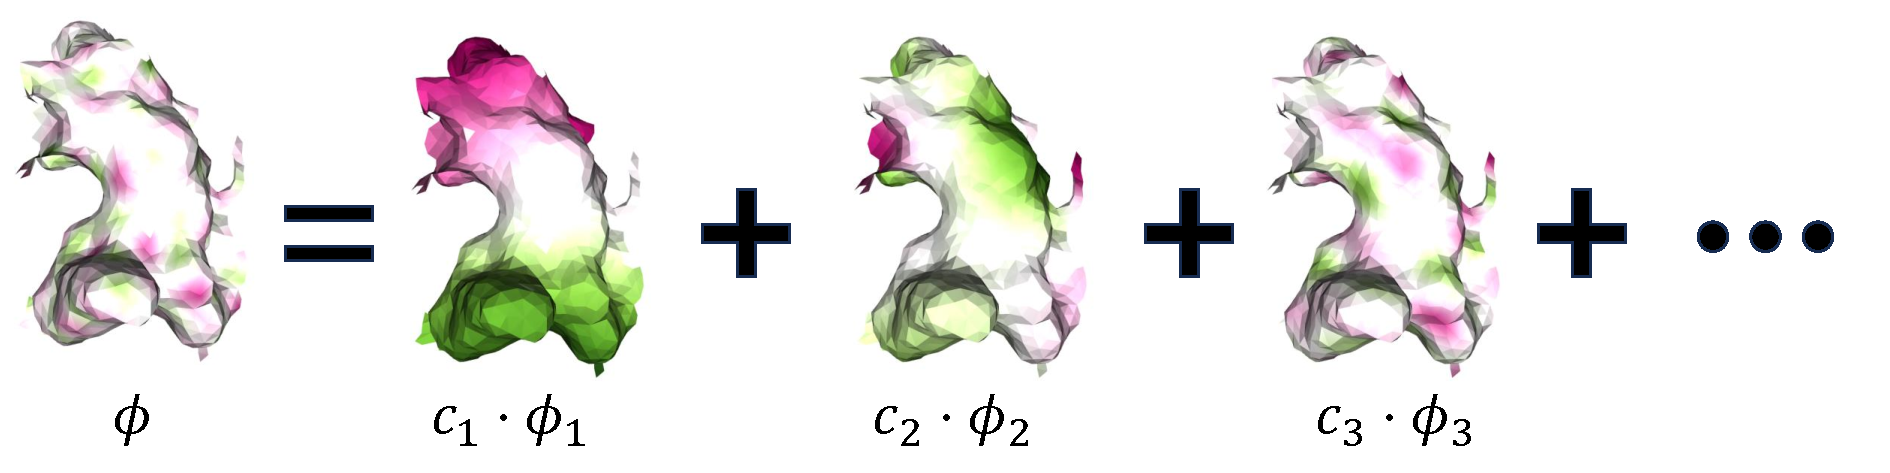
\includegraphics[width=0.7\linewidth]{figures/Laplace-Beltrami.pdf}
    \caption{
        The schematic diagram of the Laplace-Beltrami decomposition of the electrostatics field on a protein surface. It involves breaking down a continuous real-valued function $\phi$ into a linear combination of eigenfunctions $\phi_i$ with coefficients $c_i$. Eigenfunctions have varying spatial resolutions and are corresponding to distinctive details captured by them.
    }
    \label{fig:Laplace-Beltrami}
\end{figure*}
